\documentclass[11pt]{article}
\usepackage{amsmath} % AMS Math Package
\usepackage{amsthm} % Theorem Formatting
\usepackage{amssymb} % Math symbols such as \mathbb
\usepackage{hyperref}
    \hypersetup{colorlinks=true,citecolor=blue,urlcolor =black,linkbordercolor={1 0 0}}
\usepackage{graphicx}
\usepackage{caption}
%\usepackage{filecontents}
\usepackage{subcaption}% Allows for eps images
\usepackage[table,xcdraw]{xcolor}
\usepackage{tikz}
\usepackage{cite}
\usepackage{siunitx}
\usepackage{tabularx} % Allows for table with custom column width
\usepackage{lipsum}
\usepackage{parskip}
\usepackage{booktabs}
%\usepackage{mathtools}
\usepackage[letterpaper, total={6.5in, 9in}]{geometry} % see geometry.pdf on how to lay out the page. There's lots.
\usepackage [english]{babel}
\usepackage [autostyle, english = american]{csquotes}
\usepackage{siunitx}
\usepackage{float}
\usepackage{array}
\usepackage{paralist}
\usepackage{ragged2e}
\usepackage{caption}
\usepackage{graphicx}
\usepackage{lipsum}
\usepackage{url}
\usepackage{hyperref}
\usepackage{wrapfig}
\usepackage{setspace} % you can control the spacing here
\onehalfspacing
\setlength\parindent{24pt}
\MakeOuterQuote{"} % or letter or a5paper or ... etc
\usepackage{multicol} %allows you to make multiple columned items
\usepackage{verbatim}
\usepackage{xcolor}

% Setting to include lines of code. See examples in the file appendix\plotters
\usepackage{listings}
\lstset{language=Python}
\lstset{frame=lines}

\lstdefinestyle{customc}{
  belowcaptionskip=1\baselineskip,
  breaklines=true,
  frame=L,
  xleftmargin=\parindent,
  language=python,
  showstringspaces=false,
  basicstyle=\footnotesize\ttfamily,
  keywordstyle=\bfseries\color{green!40!black},
  commentstyle=\itshape\color{purple!40!black},
  identifierstyle=\color{black},
  stringstyle=\color{orange},
}
\lstdefinestyle{customasm}{
  belowcaptionskip=1\baselineskip,
  frame=L,
  xleftmargin=\parindent,
  language=[x86masm]Assembler,
  basicstyle=\footnotesize\ttfamily,
  commentstyle=\itshape\color{purple!40!black},
  }

\lstset{escapechar=@,style=customc}

\title{}
\author{}
\date{} % delete this line to display the current date

%%% BEGIN DOCUMENT
\begin{document}

\begin{titlepage}
\centering
\vspace*{0mm}
\Large{Directional Clustering -  Design Document}
\vspace{30mm}

\begin{figure}[H]
\centering

\includegraphics[scale=0.2]{images/pton .png}
\end{figure}
\vspace{30mm}
\Large{Isabel Moreira, Hui Yuan, Alexandros Papamatthaiou, Rafael Pastrana}\\

\vspace{8mm}
\large{Final Project  \\ APC524: Software Engineering for Scientific Computing \\ }
\large{Gabe Perez-Giz}\\
\large{Princeton University \\Fall 2020\\}

\end{titlepage}

% Document Skeleton

\section{Introduction}

\subsection{Motivation}

Principal stress fields are relevant to the design of volume-minimizing surface structures as they suggest optimal directions for material alignment. This implies that by following these directions, less material would be used to achieve a target level of structural performance. An example of applicability in concrete shell structures is to add steel reinforcement in the direction of tensile principal stresses so that the total amount of reinforcement needed is minimal.

Principal stress fields are ubiquitously computed by off-the-shelf finite element analysis (FEA) software and are represented as a cloud of vectors (i.e. a vector field). However, as principal stress fields are heterogeneous and form continuous curvilinear trajectories, it is actually difficult, for fabrication reasons, to place material (the reinforcement bars, beams, or other elements) in a way that exactly match the field directions (3D printing is an exception though). Therefore, extreme directional fidelity is cumbersome, and it is probably one of the reasons why we actually keep on building with crude orthogonal grids everywhere (take a look at the room around you, for example).

In this work, we question the heterogeneity of a principal stress field and inquire on how much we can simplify it so that we can maximize the feasibility of fabrication, while compromising as little as possible in structural performance. In short, what we want is to find the lowest possible amount of different vectors that encode the maximum amount of directional information about a principal stress field. We leverage a variety of clustering methods to this end.


\subsection{Scientific background}

\subsubsection{Principal stress directions}

In a material continuum subjected to in-plane external forces, principal stress directions correspond to the two orthogonal vectors that maximize normal stresses and nullify shear. Given a reference coordinate system $XY$ and a state of stress described by two normal stresses $\sigma_x, \sigma_y$ and one shear stress $\tau_{xy}$, the angle (also called "principal angle") needed to rotate it such that state of normal stress is maximized is defined by:

\begin{equation}
    \tan2\theta_{p} = \frac{2\tau_{xy}}{\sigma_x - \sigma_y}
\end{equation}

The rotated reference system $XY$ corresponds to the two principal stress directions. Similarly, the magnitude of the principal stresses $\sigma_1, \sigma_2$ is described by:

\begin{equation}
    \sigma_{1, 2} = \frac{\sigma_x + \sigma_y}{2} \pm \sqrt{(\sigma_x + \sigma_y)^2 + \tau_{xy}^2}
\end{equation}

\subsubsection{Vector field clustering}

Drawing parallels from image quantization, the directional simplification of a principal stress field is formulated as a clustering problem. The aim is to find the smallest set of vectors in $\mathbb{R}^3$ that best summarizes a principal stress field $\mathbf{F}$ within a certain distortion budget. Clustering takes place as a distance-driven process, where every principal stress vector $\mathbf{v} \in \mathbf{F}$ is assigned to the single cluster $\mathcal{C}$ whose centroid $\mathbf{c}$ is the closest.

For KMeans, the clustering process contemplates five stages: initialization, association, centroid recalculation, and termination. Let $k$ be a target number of clusters to form, $\mathbf{F}$ the principal stress field to cluster, $\mathbf{W} \in \mathbb{R}^{k \times 3}$ a matrix that stores all cluster centroids $\mathbf{c}$, and $e$ the number of epochs to run the algorithm for. To start with a reasonable estimate for  $\mathbf{W}_0$, the algorithm starts by selecting $k$ vectors $\mathbf{v}$ from $\mathbf{F}$. A loss function is introduced to evaluate the quality of the clustering with the intention to be minimized, and is defined by: 

\begin{equation}
    \mathcal{L}^{k} = \frac{1}{|\textbf{F}|} \sum^{n}_{i=1} \min_j (\mathbf{v}_{i} - \mathbf{c}_{j})^{2}
\end{equation}

Please refer to \href{https://drive.google.com/file/d/1gH3feZg796jewtrcDC3sTIwqYr9KsBPV/view}{{\textcolor{blue}{this report}}} for more details on the clustering scientific underpinnings.



\section{Software Architecture}

\subsection{Project Goals and Design Considerations}
The goal of this project is to start a modular open-source library to study the directional simplification of principal stress fields on polygonal meshes in $\mathbb{R}^3$ using different clustering algorithms. To this end, we designed the code to allow for expansion with new clustering algorithms through an Abstract Base Class and Factory Method that registers and returns the clustering algorithm of choice. This not only allows simplified extension of other algorithms in the future, but also allows multiple calls of different types of algorithms within a concise driver code that may also benefit from parallel programming in the future. Additionally, the vector field is also based on an Abstract Base Class of a general field to allow for different options of dimensionality. 
 
Another goal of the project is to provide three dimensional visualization of the clustered fields, the mesh and the underlying geometry of the structure. A desired feature is that a 3D plot with interactive visualization is provided. For this part, we dedicated a class to provide different methods of plotting options, such as line plots, mesh plots, and cone plots depending on the objective of the visualization. The ideal way to design this class is to follow the decorator pattern, where we add options of visualization on the same plot, or add subplots to view side by side. However, this specific pattern is left to future development. The current design in the code provides options through boolean flags defined in the beginning of the driver code, which are passed in to methods of the plotting class to activate the different plots.

To begin this project, we departed from Rafael's previous research work which is stored in \href{http://www.github.com/arpastrana/directional_clustering}{\textcolor{blue}{this repository}}. The previous code consisted of a small number of modules, functions, and scripts that required extensive refactoring in order to become a public library. The two most relevant functions that existed in the repository as a starting point were a custom implementation of the KMeans clustering algorithm that uses cosine distance as the basis for vector association and a simple 2D plotter for visualization. Previously, the approach relied on  \href{http://www.karamba3d.com/}{\textcolor{blue}{Karamba3d}} to extract principal stress fields. This is proprietary software, where extensions and customization would be hard to achieve, especially with the goal to turn this repository into a public library. Hence, another goal we have is to include an open source FEA package that allows us to customize functions to our needs. This part is currently a work in progress, and can be found in the $develop$ branch of the repository linked in Section \ref{section:development}.


\subsection{External dependencies}
We continue to rely on the \href{http://www.compas.dev}{\textcolor{blue}{ COMPAS }} framework as backend to handle the creation and manipulation of polygonal meshes and other geometric entities, such as circles, lines, and points. 
\href{http://www.numpy.org}{\textcolor{blue}{Numpy}} is used as the basis for all the clustering algorithms and organization of data structure. 
We have kept \href{https://scikit-learn.org/stable/index.html}{\textcolor{blue}{Scikit-learn}} as a dependency; however, we are relying only on one of its methods: pairwise distances. This dependency is intended to be replaced in future work. 

We selected the Python-based, open-source FEA \href{http://sfepy.org/doc-devel/index.html}{\textcolor{blue}{SfePy}} library.

We selected the Python-based plotting library \href{https://plotly.com/python/}{\textcolor{blue}{Plotly.py}} that is build on top of a JavaScript library (a.k.a. Plotly.js) for the visualization of results. This library is tightly integrated with
\href{https://plotly.com/dash/?utm_source=dash_demo&utm_medium=graphing_banner&utm_campaign=python}{\textcolor{blue}{Dash}}, which allows web-based applications for enhanced visualization of outputs. A more detailed perspective of this package is described in Appendix \ref{appendix:a}.

\subsection{Interfaces}

We use JSON files or COMPAS meshes to exchange output and input between each portion of the code.

We modularized the existing KMeans clustering algorithm into a generic K-means algorithm, a cosine K-means algorithm, and added Variational KMeans Clustering. Therefore, we benefited from creating an Abstract Base Class and a Factory Method that returns the clustering algorithm of choice.
The interface should allow for a call on only one type of clustering algorithm or multiple calls, each on a different algorithm. Then we should be able to compare each output in a Visualizer.


The Visualizer has as input a mesh with principal stress field and plots a 3D visualization of the vectors on the respective mesh faces. We should be able to call the visualizer multiple times to create images where we can easily compare different algorithms, or different $k$ values for one given algorithm.  

The visualizer  provides room for the user to set different views of the same output, it also leaves room for an interactive viewer that allows sliders and multiple view selections from an web-based application.



\subsection{UML Diagram}
We would like different start-points for our program. All of the enumerated options would result in MeshPlus, which will hold the mesh and principal stress vectors in such a way that we can access each one separately.
\begin{enumerate}
    \item Start point:
    \begin{enumerate}
        \item Start with a COMPAS geometry. \newline
For this option, we would generate a mesh from the geometry (through \href{https://compas.dev/plugins.html}{\textcolor{blue}{COMPAS}}), pass the mesh into an FEA solver to obtain principal stress fields and get MeshPlus.
        \item Start with FEA Solver. \newline
For this option, we would define geometry, boundary conditions, loads, and material with the given solver interface to get \emph{Our Mesh}.
        \item Start with a COMPAS mesh which already has principal stresses as face attributes and get MeshPlus.
    \end{enumerate}
    
    \item Visualize with MeshPlus with PlyPlotter and decide to continue or readjust the starting point.
    \item Continue with a clustering algorithm of our choice.
    \item Visualize the output
\end{enumerate}

These are the classes described in our UML (in Figure \ref{fig:uml}):

\begin{itemize}
    \item AbstractField
    
    Abstract base class for implementing a container of vectors
    
    \begin{itemize}
        \item Field
        
        Generic container with all entries being of a same dimension.
        
        \begin{itemize}
            \item VectorField
            
            A container for 3D vectors, storing entries with keys of the mesh they are coupled to, along with several methods for processing data it stores.
        
        \end{itemize}
    \end{itemize}
    
    \item MeshPlus
    
    Extension of COMPAS Mesh that allows storage and access of VectorField with mesh attribute, and access of attributes for all supported VectorFields in a mesh.
    
    \item FEASolver
    
    Wrapper around SfePy to simplify the structural analysis of MeshPlus and to facilitate the subsequent generation of VectorField 
    
    \item StructuralModel
    \item ClusteringAlgorithm
    
    Abstract base class for implementing clustering algorithms
    
    \begin{itemize}
        \item KMeans
        
        Generic K-means algorithm class.
        
        \begin{itemize}
            \item CosineKMeans
            
            Cosine K-means algorithm.
            
            \item VariationalKMeans
            
            Variational K-means algorithm
        
        \end{itemize}
    \end{itemize}
    \item ClusteringAlgorithmFactory
    
    A Factory with class method  that returns  the  ClusteringAlgorithm of choice.  
      
    \item PlyPlotter
    
    A 3D viewer inheriting a Figure graph object from Plotly.
\end{itemize}

\subsection{Note on FEA}

Two scripts can be found under FEA in the Finite branch of our code, which are under development. Due to time constraints, we were unable to integrate them in the driver code and they remain as scripts, not following the designed API. FEA.py takes a raw geometry file in the form of a .mesh, runs the finite-element method with the use of sfepy and outputs the u and v vectors of the mesh. The MeshCreator.py file uses the FreeCAD package to generate a mesh file out of a user specified geometry. As FEA packages usually go, both sfepy and FreeCAD have a number of dependencies that have to be met, (FreeCAD only works with Python 3.6) which made the installation process buggy and required significantly more time than originally estimated. The scripts serve as potential, workable extensions to our code, which, in the future, could allow a "from the ground up" approach, in which the clusters are received for any object specified by the user, without the use of external dependencies.  

\begin{figure}[H]
    \centering
    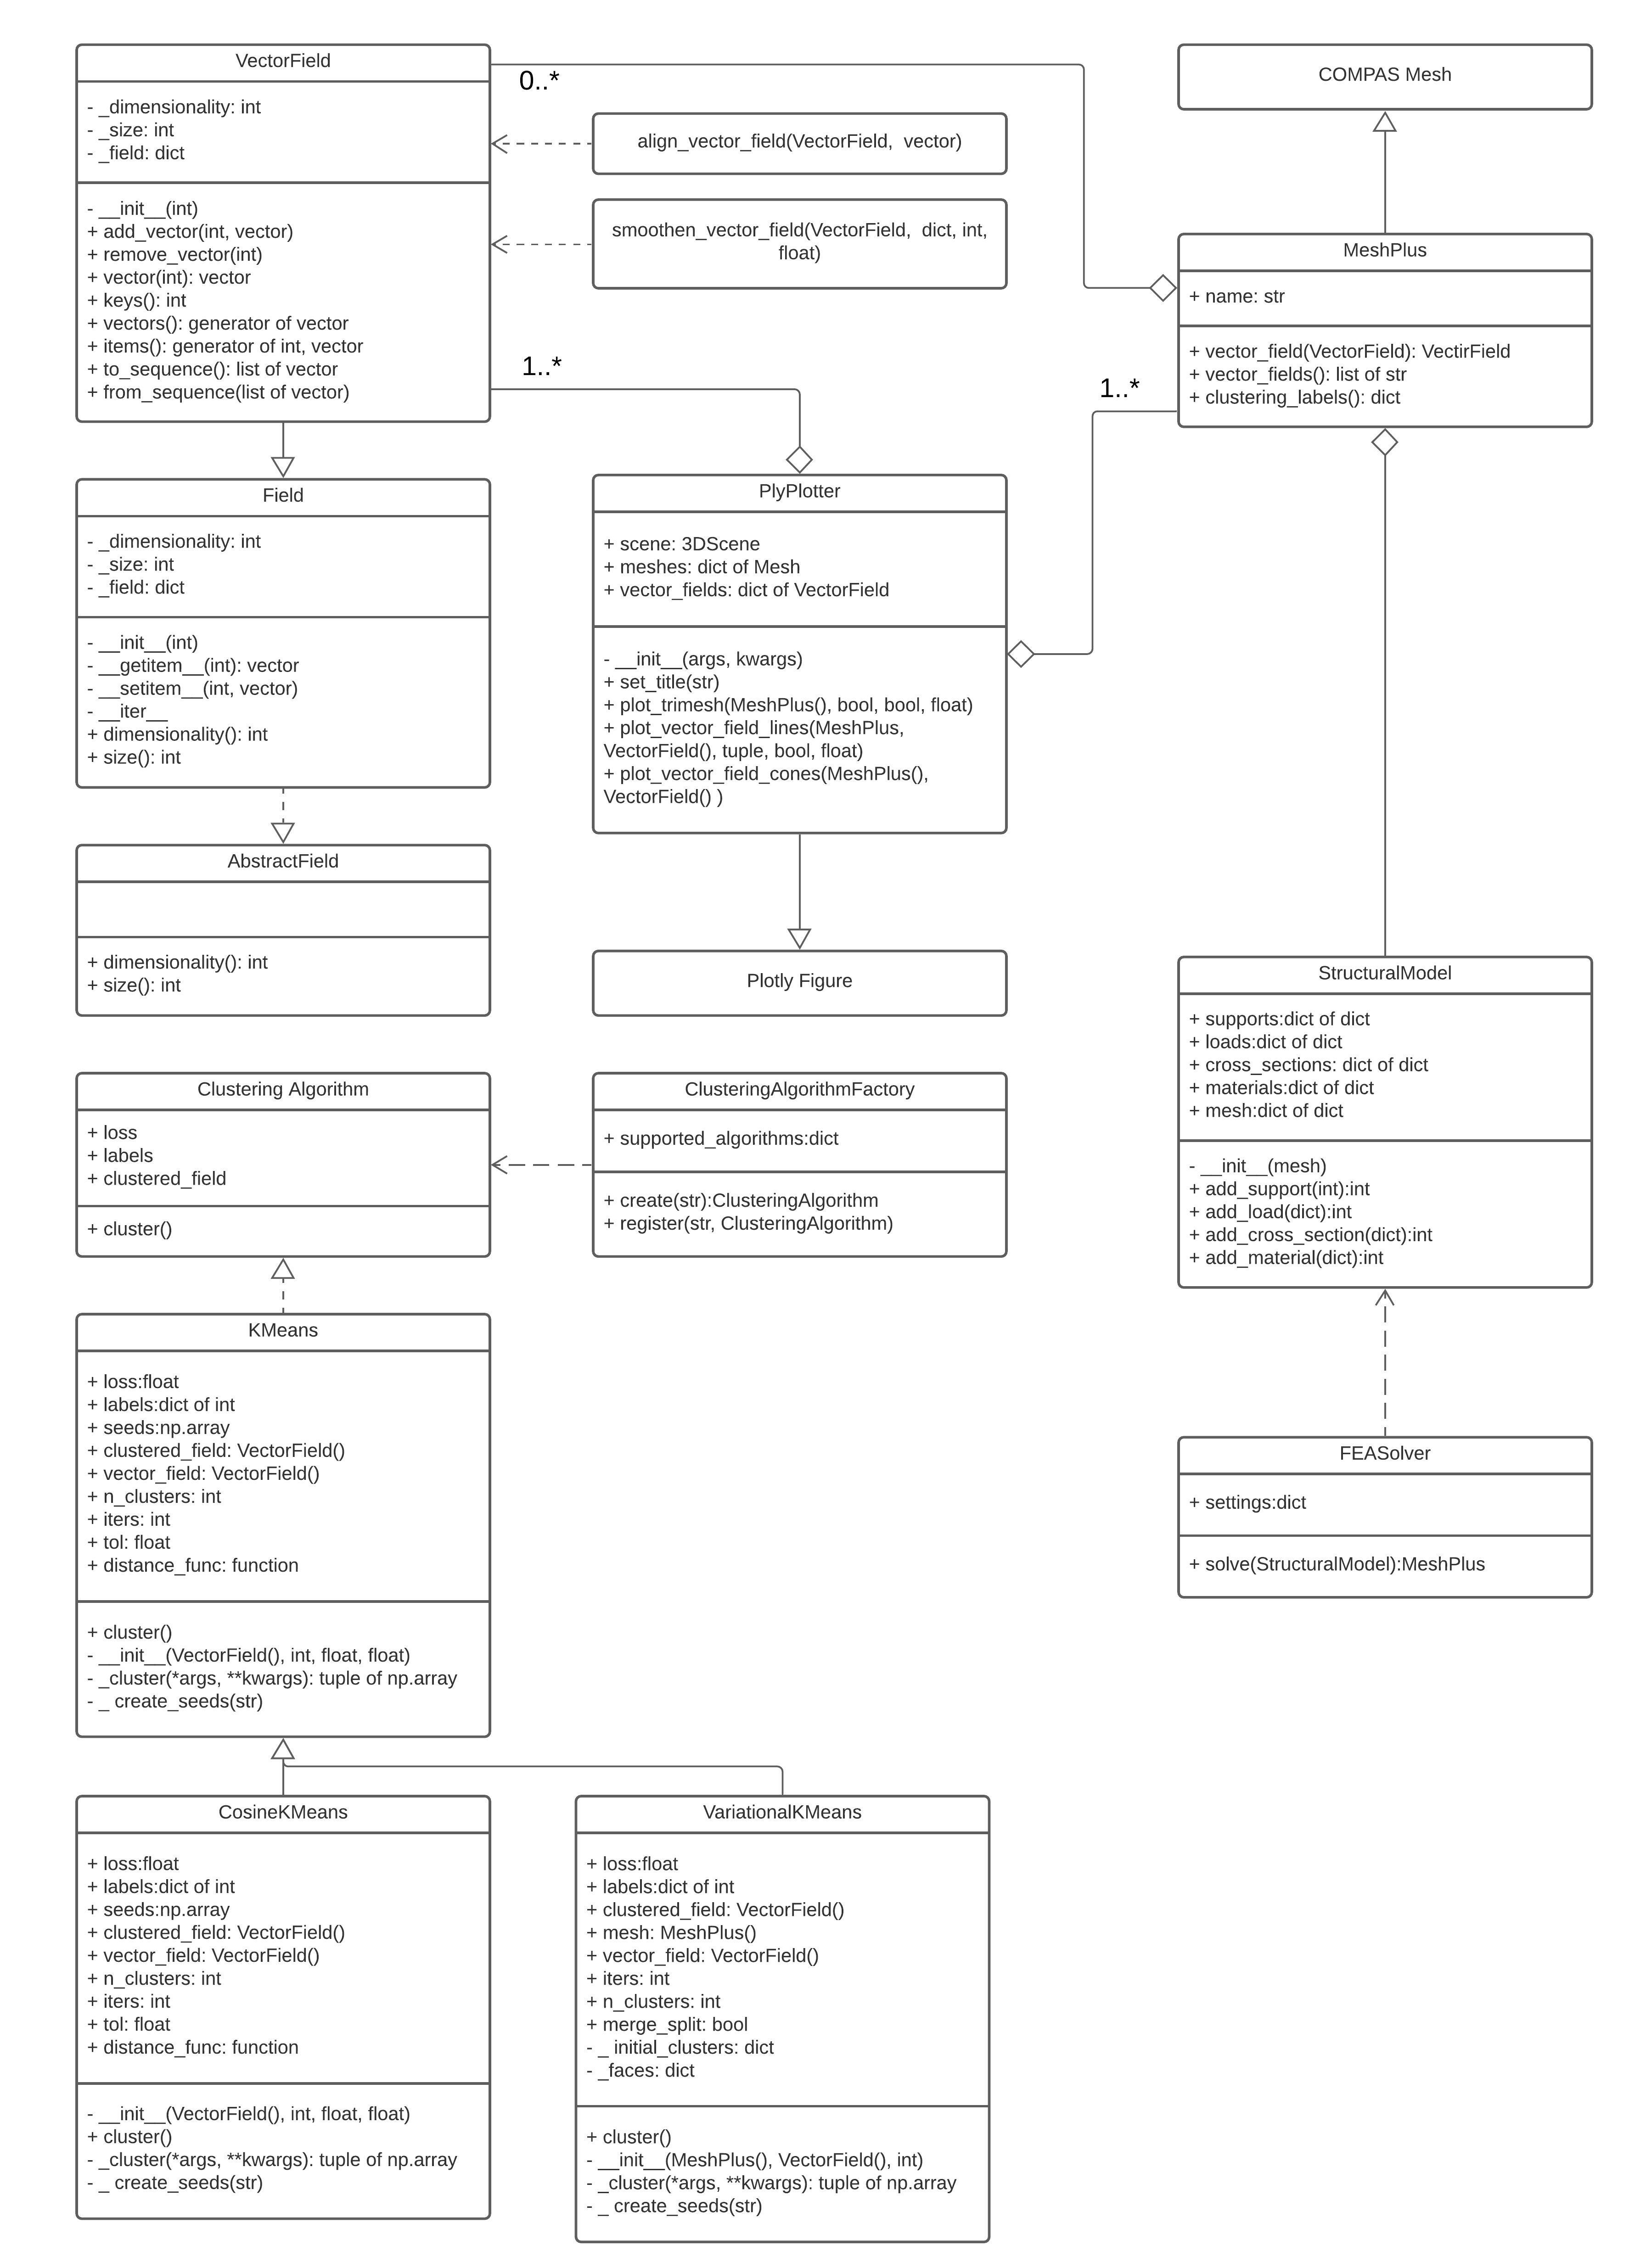
\includegraphics[scale=0.54]{images/UML-Clusters-Final.jpeg}
	\caption{UML Diagram}
	\label{fig:uml}
\end{figure}
\vspace{30mm}

\section{Development Process}
\label{section:development}

We started working on the existing repository  \href{https://github.com/arpastrana/apc524_directional_clustering}{\textcolor{blue}{apc524\_directional\_clustering}}.

We adopted Git workflow, with a centralized repository where all had writing access. We created a new repository from the one mentioned above only for the purposes of this course, and we all cloned it to local repositories. 

We kept the $master$ branch intact during our development process - which was all concentrated in the $develop$ branch. Our individual workflow was based on the following description. Before editing anything, we branched out from $develop$ to branches we named after the features we were working on. For example, we had a $vector\_field$ branch where a group member would work on a new file dedicated to adding the related class and methods. We all knew which group member had each branch because we kept similar names to the issues created in the GitHub Kanban board, where we assigned ourselves the issues we would like to work on. 
After the changes were made to the feature branch we made a pull request (PR) with a brief overview of major changes to the existing code and added or modified features and files. For each PR we had one round of review.

In the review, we questioned names of variables, making sure they would be clear to our future selves and others, we included comments related to style with PEP 8 as guide, and verified that each function had at least one test to go with it. We used PyTest to run the tests during development. After this round of review, we ran the tests in Travis CI and merged the feature branch onto the $develop$ branch if the build passed.

For the PR requests we relied mainly in one group member to review others' code, but we also took turns reviewing one round of a PR so we would all have this experience. 

We used Sphinx to build the documentation, and Overleaf to collaboratively build this final report. We would like to point out that the PlyPlotter class is currently not included in the documentation, since we would need to adjust the automatic output to bypass the documentation of the inherited class, which follows different formatting style.

Additionally, the group members worked from different countries, all in different time zones, so meetings where all group members were present were scheduled in advance with the aid of online scheduling polls, such as \href{https://www.when2meet.com/}{\textcolor{blue}{When2Meet}} and \href{https://doodle.com/en/}{\textcolor{blue}{Doodle}}. Additional meetings with only two group members were scheduled on the side. For general communication, we used Campuswire group chats in the beginning, and later we migrated to WhatsApp. For specific code-related updates, we used Kanban boards on GitHub, updating each other with new comments in the related issue.

\subsection{Profiling}
Before running the round of profiling we discussed where we expected the bottlenecks to occur. One hypothesis was that the smoothing algorithm might be taking too long to be completed because it used for-loops. The loops were used in order to make the functionality work, and it was a clear path to resolve the algorithm at the time. Another hypothesis we brought up was that the plot that generates multiple lines to visualize the vector field is also time consuming. A detailed description of ways to plot multiple lines and how to best approach this plot can be found in Appendix \ref{appendix:a}.

We had one round of profiling. The first notable result was that our driver code run for about 50-90 seconds for all attributes of the attribute matrix. Additionally, the ordering of the functions that take up the most cumulative time show no variation from attribute to attribute. The profiling software we used is cProfile, and sorted the list of 9000-9020 function calls to the top 20 of cumulative time spent. The total time taken by a function differs from the cumulative time as it includes all the time spent in sub-functions. The time per call is the total time spent in all calls over the number of calls.

\begin{figure}[H]
    \centering
    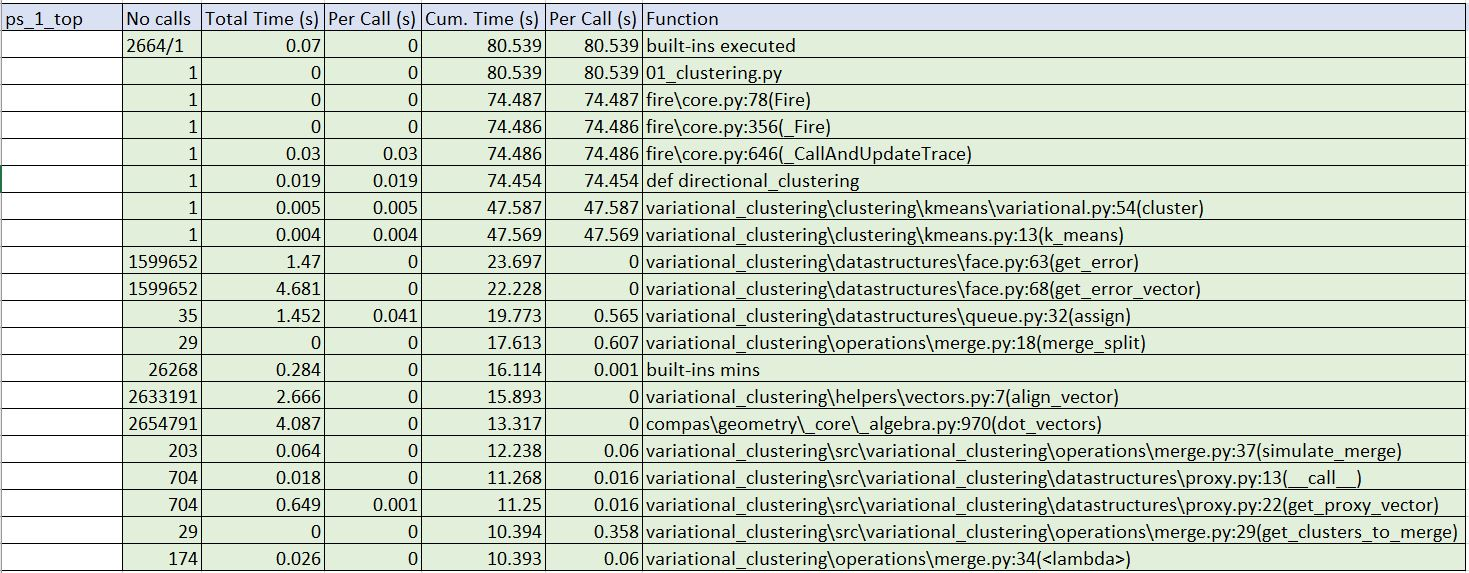
\includegraphics[scale=0.65]{Profiling.JPG}
	\caption{Profiling: cumulative time}
	\label{fig:uml}
\end{figure}

The first two calls, in terms of cumulative time, are naturally built-in Python executable and the .py file. Afterward, the fire package, which generates the text and receives commands in the CLI. The total time profile may be more informative. The add face function and the get error vector functions from variational clustering seem to be the most obvious bottlenecks in our code. They include if and for loops that generally drive up the run time. At a lower total time, the align vectors function also drives up the run time. Apart from variational clustering, the compas geometry files are also costly. The profiling is done on the driving code, clustering.py. The plotters.py code demonstrates a total run time between 5-10 seconds, with the 10-20 in the top 20 in total time taking up less than 0.1s.

\begin{figure}[H]
    \centering
    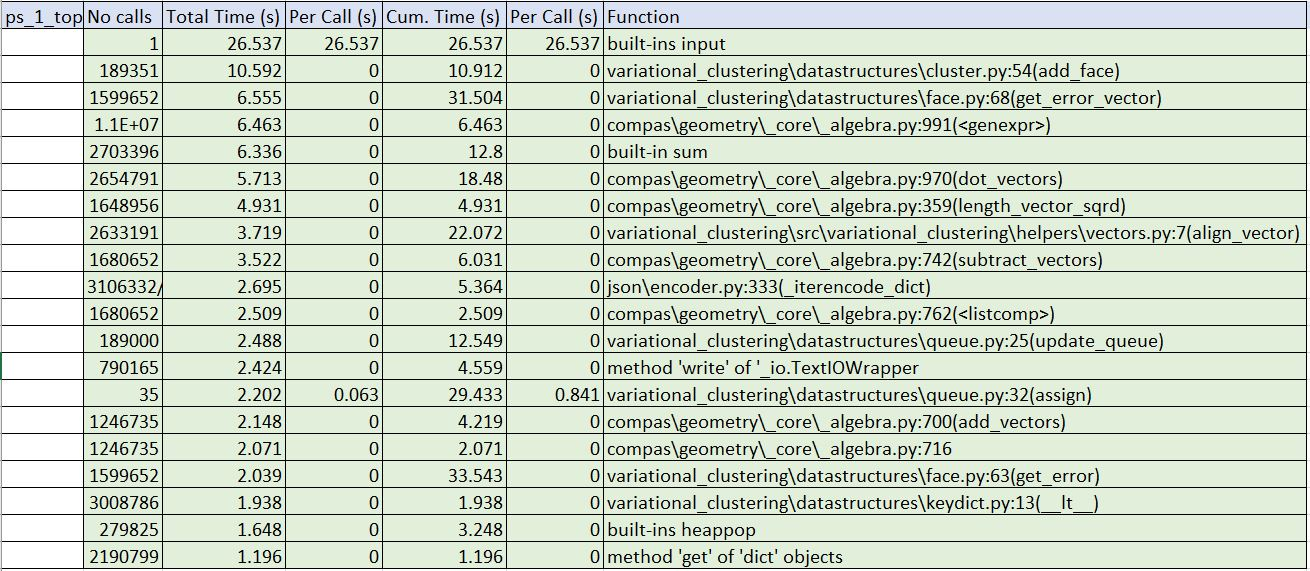
\includegraphics[scale=0.65]{Profiling2.JPG}
	\caption{Profiling: total time}
	\label{fig:uml}
\end{figure}


\subsection{Lessons learned}

As a group, we were able to discuss several lessons learned, where one of the continuous challenges we faced was to schedule meetings that were in a good time for everyone. Between Mexico, USA East Coast (and later Greece), Brazilian South East, and Chinese East we were were left with few options where all had to compromise regular working hours to be able to meet. The group worked with different channels of communication to find the best way to keep each other up to date with the development process and what to do next.

While we relied on a central group member to refer to with question on the existing code we started from, we also learned it was important to keep strong communication between each other. We found that format compatibility between functions/features can be a challenge, and we leave a few data compatibility issues to be resolved and developed in the future.

Additionally, starting early is another topic we brought up in our final group meeting. This is important not only for compatibility between different parts of the code, but also to allot time for unexpected bugs in third party packages.

We also found that detailed PR reviews are a great way to learn, both as reviewer and “reviewee”. When the code is being reviewed it is great to have constructive comments where we are pointed to style guide sections we might not have given proper attention, or variables with confusing names, or how to best describe the function in documentation. As a reviewer, it was an opportunity to learn how to read through others’ code critically and to think how it is all functioning as an addition or alteration to the existing code.


\section{Future Work}

We outline a number of directions to extend to this project further. First, enlarging the proposed library of clustering algorithms would be of genuine interest. In the future, would like to generate a driver code that takes advantage of parallel runs of different clustering algorithms and exports multiple types of plots to provide visualization of the data and compare results. Another possibility would be to run multiple meshes through the algorithm, this way, we could compare meshes with different boundary conditions or loads.

We are also leaving as future work to solve the data compatibility between the FEA solver and the expected mesh input to the clustering algorithms. 

Additionally, with the newly incorporated plotter, we would like to extend the custom plots capabilities to many other types of visualization, including an extension to a web-based app where different types of plot can be seen and compared.
Before extending the plotter, though, we would benefit from refactoring the current class to the Decorator design pattern. 
We are also looking forward to complete any missing documentation and tests.

Lastly, we envision to eventually make this package an official plugin of the \href{http://www.compas.dev}{\textcolor{blue}{COMPAS}} framework.


\clearpage
\appendix

\section{Plotters}
\label{appendix:a}

% This is where we describe the process to choose the Plotter package

\subsection{Introduction}
The main objective of this section is to implement a 3D viewer to replace the current 2D viewer. 

\subsubsection{Objectives}
\begin{itemize}
    \item Implement a 3D viewer that allows us to add layers of geometry and compare multiple outputs
    \item Open the possibility for an interactive viewer in the future
    \item Open the possibility for web applications to visualize results
\end{itemize}

After looking into several options of packages we chose to use \href{https://plotly.com/python/}{\textcolor{blue}{Plotly.py}}. 

\subsubsection{Reasons for selecting Plotly}
\begin{itemize}
    \item "The Plotly Python library is an interactive, open-source plotting library"
    \item It is "Built on top of the Plotly JavaScript library (plotly.js)"
    \item It also enables creation "of interactive web-based visualizations that can be displayed in Jupyter notebooks and saved to standalone HTML files"
    \item It an be extended to serve "as part of pure Python-built web applications using Dash." This option includes animations and visualizations of multiple outputs with sliders.
    
Citations from \href{https://plotly.com/python/getting-started/}{\textcolor{blue}{Plotly.py - getting started}}.
\end{itemize}

\subsection{Learning how to use the package}

The plots usually expect separate lists of $x$, $y$ and $z$ coordinates, and not a list of 3D points with $(x, y, z)$ coordinates, like the ones we are using with the COMPAS package. So the first job here was to separate the data according to what is expected for each plot. Helper functions were defined in a separate folder to do this job.

\subsubsection{Graph objects}

\begin{lstlisting}
import plotly.graph_objects as go
\end{lstlisting}

This module allows for many types of plots, such as \emph{3D Meshes}, \emph{3D Scatter}, and vector fields as directed \emph{Cones}. 

The visuals of the vector field viewer with directed cones is pleasing, and the impression is that the plot builds quickly. However, the current objective of the vector field visualization is not to see a preferred direction, but only the line in which it describes from the related face centroid.

For that, we can use the 3D Scatter plots with the \emph{mode} set to \emph{lines}. And here comes the interesting part of the line visualization... It was not obvious at first how to display many lines in one plot. Plotly uses \emph{traces} as a list of each set of point to create line plots. The first reference found suggested building loops to create many different \emph{traces} and plot all of them as \emph{data} (a list of \emph{traces}). But that option takes an extremely long time with the extensive amount of lines we desire to plot, and it's simply not an option. After more rounds of exploration, the solution found is to build three empty lists (one for each coordinate) (\lstinline{np.empty(3 * number of lines})  and fill them  with the corresponding start and end coordinate for every first and second positions every 3 positions, like so:

\begin{lstlisting}
list_x = np.empty(3 * num_lines)
list_x[::3] = start_x
list_x[1::3] = end_x
list_x[2::3] = None
\end{lstlisting}
The same is repeated for $y$ and $z$ coordinates.

This way, we inform the plotter points to be connected are the points that have a number inside, and that no line will connect the end point of one line with the start point of the next because of the inserted separator.

Another plotter explored in the package was 3d Mesh. One limitation is that the this plot doesn't have an option to display the mesh edges as lines - so we can't see the triangulation clearly. Another limitation is that it can only display triangulated meshes. For now, in this project, we are only working with triangulated meshes and this is not a problem. In the future, though, if we wish to display other polygonal meshes, then we may be forced into triangulating it for display. One possible solution is to display mesh edges to repeat the line process described above. Another solution found is to show the edges with the module described below.

\subsubsection{Figure Factory}

\begin{lstlisting}
import plotly.figure_factory as ff
\end{lstlisting}

With this plotting option we can include the lists of coordinates of the mesh vertices and the corresponding indices that build each triangular face of the mesh - called simplices (again, only for triangulated meshes). The problem here is that the automatic color function setting uses $z$ coordinates to calculate color tone, and if your input has all $z$ coordinates lined up, then it throws an error that it can't calculate the distance between vertical points. The way to bypass this is to set another color function. In our case it was very simple, we just selected the color attribute of COMPAS mesh faces: \lstinline{color_func=list(face_colors.values())}. 
In case this colorful view is not desired, then the option provided is to generate a list with the same length as mesh faces with one color repeatedly. 






\end{document}
